\begin{ccRefConcept}{ConformPolicy_2}

\ccDefinition

The concept \ccRefName{} describes the way the
\ccc{Conform_triangulation_2<CDT>} class conformes its edges. It is
used by the templated method
\ccc{Conform_triangulation_2<CDT>::conform(ConformPolicy)}, in which
the template parameter \ccc{ConformPolicy} must be a model of
\ccRefName{}.

To resolv a circular dependancy problem, the two types of this concept 
are templated by the triangulation class itself.

\ccTypes

\ccTypedef{typedef CDT::Face_handle Face_handle;}{The \ccc{Face_handle}
  of the triangulation.}

The following predicate class tests if an edge of the triangulation is
\emph{locally conform}. Given a meaning to \emph{conform},
\emph{locally conform} means that, if all edges of the triangulation
are \emph{locally conform}, then they are both \emph{conform}. An edge
can be \emph{locally conform} without being \emph{conform} if some
other edges of the triangulation are not \emph{locally conform}.

\ccNestedType{template <class CDT> Is_locally_conform} { Must provide
  the operator \ccc{bool operator()(const CDT& t, Face_handle fh, int
    i)} that tells if the edge (fh,i) is \emph{locally conform}.}

The following predicate class tests if a face of the triangulation
like in figure \ref{part_of_a_cluster} can be part of a cluster or its 
two edges cannot be in the same clusters. \todo{Ce concept est \`a la
  fois foireux et difficile \`a expliquer.}

\begin{figure}
\begin{ccTexOnly}
\begin{center}
\includegraphics{Mesh_2_ref/part_of_a_cluster.eps}
\end{center}
\end{ccTexOnly}
\caption{A face part of a cluster}
\label{part_of_a_cluster}
\begin{ccHtmlOnly}
<CENTER>
<img border=0 src=part_of_a_cluster.gif align=center alt="Face part of
a cluster">
</CENTER>
\end{ccHtmlOnly}
\end{figure}

\ccNestedType{template <class CDT> Is_acceptable_in_a_cluster<CDT>;}{
  Must provide the operator \ccc{bool operator()(const CDT& t,
    Face_handle fh)} that tells if the face fh is acceptable. }

\ccCreation
\ccCreationVariable{policy}

\ccConstructor{ConformPolicy_2();}{default constructor.}

\ccHeading{Access to predicate and constructor objects}
\ccMethod{template <class CDT>
          Is_locally_conform<CDT>
          is_locally_conform_object();}{}
\ccMethod{template <class CDT>
          Is_acceptable_in_a_cluster<CDT>
          is_acceptable_in_a_cluster_object();}{}

\ccHasModels
\ccc{Gabriel_conform_policy_2} is the policy class that permit to
conform edges according to the Gabriel criteria.

\ccc{Delaunay_conform_policy_2} is the policy class that permit to
conform edges according to the Delaunay criteria.

\ccc{Gabriel_conform_inside_policy_2} is a special policy used by
\ccc{Mesh_2<CDT>}. An edge is encroached only if its diameter circle
intersected by the interior of the domain containts points visible
from the edge.

\todo{Documenter ces trois policies un peu mieux.}



\end{ccRefConcept}